\documentclass[a4paper]{article}
\usepackage[T1]{fontenc}
\usepackage[utf8]{inputenc}
\usepackage{lmodern}
\usepackage{graphicx}
\usepackage[left=2.5cm,right=2.5cm,top=3cm,bottom=3cm]{geometry}
\usepackage{eurosym}
\usepackage{fancyhdr}%encabezado y pie de página
\usepackage[colorlinks=true, linkcolor=black, urlcolor=blue]{hyperref}
\setcounter{secnumdepth}{5}
\usepackage[spanish]{babel}
\setcounter{tocdepth}{5}
\usepackage{colortbl}%para colorear tablas
\usepackage{tabularx}
\usepackage{placeins}%para poner barrera y no pasen de secciones los elemntos flotantes
%\usepackage{wasysym} %para poner símbolos
\usepackage{bbding} %para poner símbolos



%para el mapa mental
\usepackage{tikz}
\usetikzlibrary{mindmap,trees}
\usepackage{verbatim}


\date{}
\author{D. Ramirez Ambrosi \\ J. I. Sánchez Méndez \\ J. Rodríguez Azpeleta}
\title{\begin{center}
\textbf{\Huge{Make Yourself Strong}} \\ Análisis de necesidades  \\Proyecto de la asignatura Interacción Persona Computador \\ \Huge{Grupo 10}
\end{center}}
\date{\today}


\pagestyle{fancy}
\rhead{
\textbf{Make Yourself Strong} \hfill \textbf{Fecha:} \date{\today}
}

\lhead{}

%Separación entre párrafos
\setlength{\parskip}{3mm}

%colores
\definecolor{verde}{RGB}{127,255,0}%color para la barra de titulo
\definecolor{rojo}{RGB}{255,0,0}%color para características
\renewcommand\listfigurename{\centering LISTA DE FIGURAS}

\begin{document}
\maketitle

\thispagestyle{empty}%para evitar enumeración de la página de la portada y del índice
\newpage
\tableofcontents%índice
\thispagestyle{empty}
\newpage



%lista de figuras 
%\renewcommand\listfigurename{\centering LISTA DE FIGURAS}
%\listoffigures
%\clearpage

%Lista de tablas
%\renewcommand{\listtablename}{\centering ÍNDICE DE TABLAS} %Para cambiar el índice de las tablas
%\listoftables
%\thispagestyle{empty}
%\newpage

\setcounter{page}{1}%Para reinizar el contador de páginas en la página deseada


\section{Introducción}

La prueba está basada en el uso de la aplicación \textbf{MyFitnessPAL} \footnote{\url{http://www.myfitnesspal.com.mx}}. Esta aplicación está centrada en la cuenta de calorías de un usuario. En base a parámetros - como la altura, peso y nivel de actividad física - y objetivos - como mantener o variar el peso - muestra una estimación de las calorías que el usuario debe consumir al día así como la cantidad de macronutrientes (hidratos de carbono, grasas y proteínas) que debe consumir para alcanzar los objetivos deseados.

Los usuarios pueden realizar el seguimiento calórico mediante el registro de los alimentos consumidos mediante búsquedas en la base de datos propia. También tienen la posibilidad de añadir un alimento en caso de no encontrarlo en dicha base de datos.

También tienen la posibilidad de registrar las calorías consumidas por ejercio físico. Como en el caso anterior, se puede buscar el ejercicio en la base de datos o añadirlo en caso de que no se encuentre.

Los usuarios pueden realizar su propio seguimiento mediante la consulta de estadísticas gráficas.

\section{Observación de participantes}

	\subsection{Jonathan Castro}
	
	Estudiante de Ingeniería informática, práctica deporte de forma regular.
	
		\subsubsection*{Registro de usuario}
		
		Llevado a cabo sin mayores dificultades. Resultó molesto que se pidiera información como la fecha exacta de nacimiento - Con el año para el cálculo de la edad serviría - así como el código postal y ciudad de residencia.
		
		Durante el registro se pregunta sobre los objetivos, las descripciones del nivel de actividad no resultan muy descriptivas. Además, no determinan de forma clara si en ese nivel de actividad se incluye el que se haga ejercicio regularmente o únicamente trata el nivel de actividad habitual referente a la profesión de la persona.
		
		\subsubsection*{Añadir un entrenamiento}
		
		Tras añadir un entrenamiento, se muestra en una tabla. Se da la opción de eliminarlo, aunque no se ve claramernte está función ya que viene representada por un icono con una señal de prohibición. Un icono más representativo de la función eliminar evitaría confusiones.
		
		En el caso de añadir un entrenamiento de fuerza, solo se puede añadir para un entrenamiento determinado un número de series con el mismo peso y repeticiones para cada una de las mismas. En este caso se hubiera querido especificar el peso y repeticiones para cada serie concreta.
		
		Al contabilizar las calorías quemadas en el entrenamiento, se muestran solo las correspondientes al entrenamiento cardiovascular y no se tienen en cuenta las del entrenamiento de fuerza.
		
		Otro defecto fue que las estimaciones de las calorías no eran exactas en determinados entrenamientos.
		
		Una sugerencia en este apartado fue que se tuvieran en cuenta patologías que el usuario pudiera tener para que la aplicación pudiera indicar si se daban casos de sobreesfuerzo.
		
		\subsubsection*{Añadir alimentos}
		
		En general, ningún defecto en cuanto a la interacción. El problema viene de la estimación dada para algunos alimentos
		
		\subsubsection*{Comentarios y mejoras generales}
		
		Estimaciones, tanto en calorías de los entrenamientos, como de macronutrientes de los alimentos y estimación de objetivos.
		
		En cuanto a menús, los botones de sesión, menos destacados que el resto, quedan poco a la vista. El calendario para selección de fechas está en formato inglés, siendo domingo el día que se encuentra en primer lugar.
		
			\begin{figure}[!h]
				\centering
				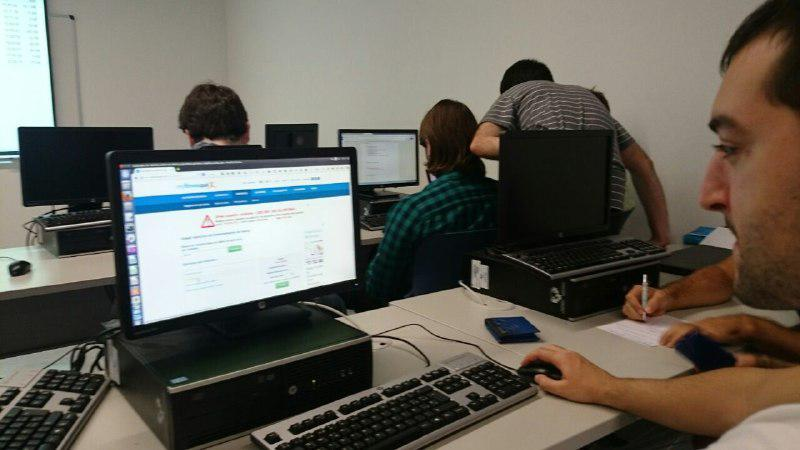
\includegraphics[width=0.7\textwidth]{./figuras/jonat-1.jpg}
				\caption{}
			\end{figure} 
		
			\begin{figure}[!h]
				\centering
				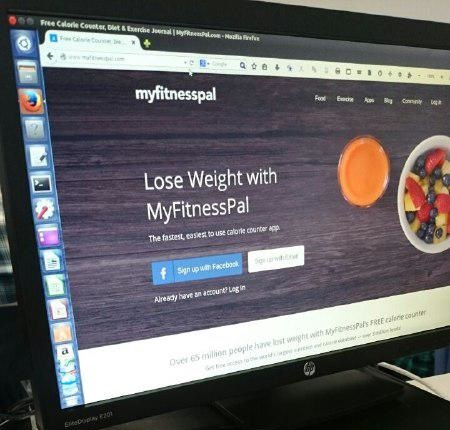
\includegraphics[width=0.5\textwidth]{./figuras/jonat-2.jpg}
				\caption{Página principal}
			\end{figure} 
			
			\begin{figure}[!h]
				\centering
				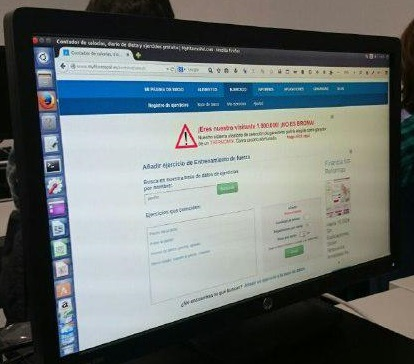
\includegraphics[width=0.5\textwidth]{./figuras/jonat-3.jpg}
				\caption{Añadiendo un ejercicio de fuerza}
			\end{figure}
		
		\FloatBarrier
		
		\subsection{Marta Aguilera}
		
			\subsubsection*{Registro de usuario}
			
			\subsubsection*{Añadir un entrenamiento}
			
			\subsubsection*{Añadir alimentos}
			
			\subsubsection*{Comentarios y mejoras generales}
			
		\FloatBarrier
		
		\subsection{Andoni Martín}
		
			\subsubsection*{Registro de usuario}
			
			\subsubsection*{Añadir un entrenamiento}
			
			\subsubsection*{Añadir alimentos}
			
			\subsubsection*{Comentarios y mejoras generales}
			
		\FloatBarrier
		

\section{Necesidades identificadas}

A continuación se detallan las diferentes necesidades detectadas en las diferentes observaciones.

	\subsection{Descripciones de elementos}
	
	Las descripciones que se asocien a diferentes elementos de una lista de opciones tienen que ser lo suficientemente claras para que el usuario no tenga ninguna duda de cuál es la que le conviene marcar.
	
	Este problema se da en el caso de la selección de la actividad diaria realizada donde se ejemplifica cada opción con una profesión pero no queda claro si se incluye la actividad física no asociada a la profesión que la persona pueda realizar.
	
	\subsection{Estimaciones más exactas}
	
	En general, ya sea al estimar los objetivos del usuario, las calorías y macronutrientes asociados a un alimento o las calorías consumidas por un determinado ejercicio, procurar, en la medida de lo posible, ofrecer valores más exactos al usuario.
	
	\subsection{Localización del usuario}
	
	En el caso del calendario, su formato era inglés. De cara a ofrecer un mejor servicio, se debería adaptar el calendario o incluso las unidades de medida al sistema utilizado en el lugar desde el que el usuario realiza la conexión.
	
	\subsection{Iconos representativos}
	
	En el caso de funciones básicas como eliminar un elemento, añadirlo o modificarlo, no se puede dar lugar a dudas de la acción representada por el icono en cuestión.
	
	\subsection{Registro de entrenamientos más preciso}
	
	Permitir especificar para un ejercicio de fuerza las diferentes series de forma individual, con un peso y repeticiones concretos para cada serie.
	
	\subsection{Registro de patologías}
	
	Permitir al usuario problemas que padezca (asma, problemas de corazón, dañoos musculares...), de forma que la aplicación avise en caso de sobre esfuerzo en base a los ejercicios añadidos a un entrenamiento.
	
	\subsection{Destacar los botones de sesión}
	
	Hacer que sean perfectamente visibles para que el usuario encuentre fácilmente, por ejemplo, el cierre de sesión.



\end{document}